\chapter{Solución propuesta}
\label{solucion}
Hoy por hoy el desarrollo de Internet ha alcanzado niveles realmente impresionantes, no solo en lo que respecta a avances en capacidad de transmisión y almacenamiento de datos sino también en su modelo de crecimiento y expansión en la sociedad post-moderna en la era de de la información. Prácticamente no hay rincón del planeta en donde no pueda hoy en día llegar la red de redes.\\

\section{Arquitectura de la solución}
\label{arquitectura}
De acuerdo al problema planteado y a los requerimientos especificados, es esencial implementar un sistema que pueda difundirse en la sociedad de manera masiva y veloz. La RedSolLAC quiere y debe poder llegar al mayor número de personas interesadas en producir energías limpias lo mas próximo en el tiempo.\\

Actualmente la RedSolLAC solo cuenta con un sitio Web donde publica información respecto de plantas solares productoras de energía, sin embargo con el objetivo de expandir sus alcances, objetivos y adherir miembros a la red, es que requiere de nuevas herramientas atractivas para los futuros integrantes. Es acá donde la presente memoria interviene, para desarrollar un nuevo sistema que integre el sitio Web ya existente con nuevas componentes que marquen la diferencia.

Para dar cumplimiento a los requerimientos especificados se propone el siguiente Diagrama General de Arquitectura:

\begin{figure}[h!]
        \centering
        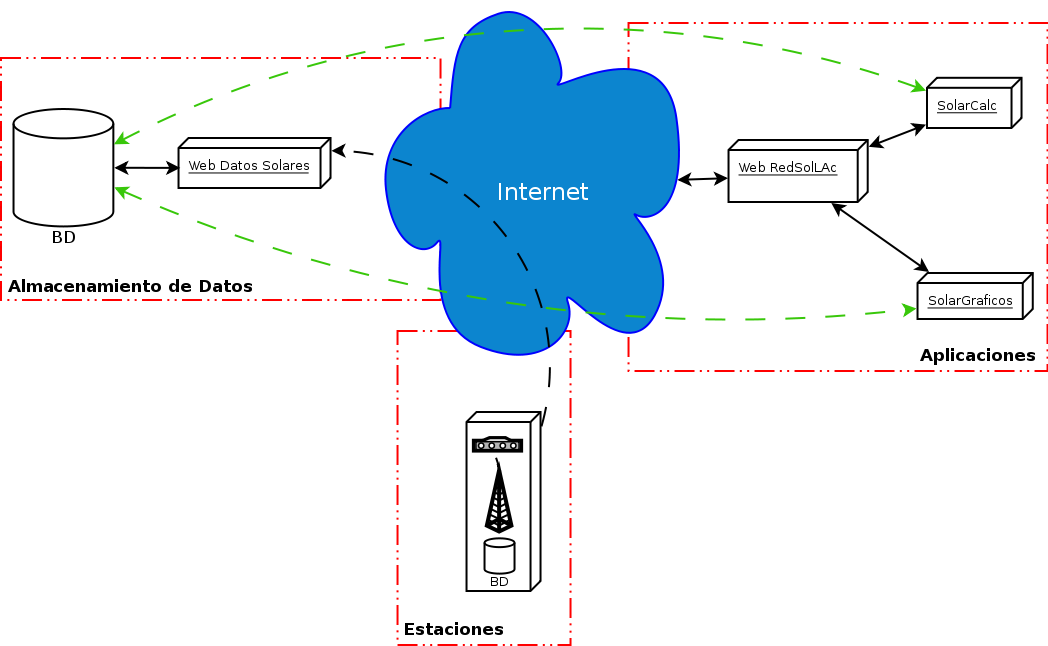
\includegraphics[width=300pt]{images/diagramaArquitectura}
        \caption{Diagrama general de arquitectura}
	\label{da}
\end{figure}

En el diagrama(Fig:\ref{da}) apreciamos las 3 partes que componen el nuevo sistema desarrollado, en primer lugar la componente de "Aplicaciones", el cual consiste en un servidor Web que implementa la plataforma CMS Wordpress. Bajo esta plataforma se desarrollan las aplicaciones principales del sistema, las cuales seran visitadas por los usuarios finales. Las "Estaciones", que son parte fundamental del proceso de adquisición de datos en el sistema,  a estas se les debe integrar un sistema de comunicación compatible con la plataforma de almacenamiento de datos. Finalmente la componente de "Almacenamiento de Datos", la cual consiste en un servidor Web que administra los procesos de registro, acceso y mantención de datos y un servidor de base de datos. Cada una de estas partes debe interactuar con las demás de manera muy precisa para conseguir el comportamiento requerido.\\

A continuación se describen las diferentes herramientas tanto de hardware como de software que implementa el sistema:

\subsection{Sofware utilizado}
\subsubsection{Wordpress}
Wordpress es una avanzada plataforma semántica de publicación en la Web. Libre, de código abierto y gratuito con altos estándares de diseño y usabilidad. Es un sistema de manejador de contenidos (\gloss{cms}) basado en estilo de publicaciones de blogs, además se distribuye bajo la licencia GPL2. Está echo en lenguaje PHP, utiliza el motor de bases de datos MySql y hojas de estilo CSS para la parte visual. Su arquitectura está pensada y diseñada de forma modular, lo que le permite adaptarse y ser configurable de acuerdo con los requerimientos de cada usuario.\\
La primera versión fue liberada el año 2003 por Matt Mullenweg y es un rama del otro proyecto llamado b2/cafelog. Actualmente esta plataforma está en su versión 3.0. Se estima que Wordpress a la fecha es la herramienta de publicación de contenido más utilizada y popular de la Red, con aproximadamente un 14\% de participación en Internet y con más del 22\% de utilización sitios nuevos o que se publican por primera vez.

Wordpress está echo de tal manera que permite a sus usuarios modificar o configurar partes esenciales del sistema, lo que lo hace flexible para agregar funcionalidades y adaptarse a los requerimientos de los usuarios. Además cuanta con un framework y una \gloss{api} que facilita la labor de los programadores.\\

Algunas caracteristicas especificas de wordpress son:

\paragraph{Perfil Gráfico}	
La parte visual de esta plataforma funciona a través de un sistema llamado \gloss{themes}(para efectos prácticos en adelante "Perfiles"). Los "Perfiles" son un conjunto de \gloss{bibliotecas} programadas en PHP y JavaScript que permiten organizar la forma en que se presentan los contenidos del sitio sin alterar el contenido. Wordpress al estar diseñado de manera modular, permite a sus usuarios contar con gran cantidad de "Perfiles" diferentes. Mediante una interfaz de administración permite cambiar estos "Perfile" de manera rápida y sencilla. Adicionalmente en el mercado, existen extensos depósitos de "Perfiles" que pueden ser instalados en cualquier sitio compatible con la versión indicada por el creador.

En el sitio de Wordpress se puede encontrar una extensa documentación y una API que indica a los programadores que deseen desarrollar nuevos "Perfiles", cómo deben estructurar los ficheros y qué funcionalidades pueden agregar o quitar. Adicionalmente los "Perfiles" pueden publicarse o bien Wordpress da la libertad a sus usuarios de vender trabajos basados en su framework.\\

\paragraph{Plugins}
Los \"\gloss{plugins}\"  funcionan casi de la misma manera que los \"Perfiles\" y así también la mayoría de los componente que dispone Wordpress. Estos son un conjunto de bibliotecas programadas en PHP y JavaScript que pueden instalarse o desinstalares desde el panel de administración.\\
Cada "Plugin" está diseñado para agregar nuevas funcionalidades o modificar el comportamiento normal de los sitios, la documentación de Wordpress entrega pautas estrictas de cómo deben estar programadas las bibliotecas para que las nuevas funcionalidades no interfieran con el funcionamiento normal del sistema.

\paragraph{Widgets}
Los \"Widgets\" son pequeños programas autónomos que permiten agregar nuevas funcionalidades al sistema, pero que a diferencia de un \"Plugin\" común y corriente posen una interfaz visual y están diseñados para exponer al usuario algún dato o funcionalidad específica. Estos pequeños programas pueden agregarse y quitarse de manera muy rápida y pueden y tienen la característica de ser móviles. Generalmente son programas que se agregan en las barras laterales.

\paragraph{Multiusuario}
Wordpress permite la creación y administración de muchos usuarios, los cuales pueden tener diferentes responsabilidades dentro del sistema, tales como administrar el contenido o bien la configuración del sitio. Esto permite que la mantención del sitio y a la vez las responsabilidades, puedan estar muy bien distribuidas sin riesgo de que algún usuario realice tareas no permitidas por su nivel de acceso.

\subsubsection{PHP}
PHP es un acrónimo recursivo que significa PHP Hypertext Pre-processor. Fue creado originalmente por Rasmus Lerdorf en 1994; sin embargo, la implementación principal de PHP es liderada , en la actualidad, "The PHP Group\cite{php:1}" y sirve como el estándar de facto para PHP al no haber una especificación formal. Publicado bajo la PHP License, la Free Software Foundation considera esta licencia como software libre.\\

Es un lenguaje de programación interpretado de alto rendimiento, diseñado originalmente para la creación de páginas web dinámicas. Se usa principalmente para la interpretación del lado del servidor (server-side scripting), pero actualmente puede ser utilizado desde una interfaz de línea de comandos o en la creación de otros tipos de programas incluyendo aplicaciones con interfaz gráfica. Sus características principales son:

\begin{itemize}
\item Orientado al desarrollo de aplicaciones web dinámicas con acceso a información almacenada en una base de datos.
\item El código fuente escrito en PHP es invisible al navegador web y al cliente, ya que es el servidor el que se encarga de ejecutar el código y enviar su resultado HTML al navegador. Esto hace que la programación en PHP sea segura y confiable.
\item Capacidad de conexión con la mayoría de los motores de base de datos que se utilizan en la actualidad, destaca su conectividad con MySQL y PostgreSQL.
\item Capacidad de expandir su potencial utilizando módulos.
\item Posee una amplia documentación en su sitio web oficial, entre la cual se destaca que todas las funciones del sistema están explicadas y ejemplificadas en un único archivo de ayuda.
\item Es libre, por lo que se presenta como una alternativa de fácil acceso para todos.
\item Permite aplicar técnicas de programación orientada a objetos.
\item Amplia biblioteca nativa de funciones.
\item No requiere definición de tipos de variables aunque sus variables se pueden evaluar también por el tipo que estén manejando en tiempo de ejecución.
\item Tiene manejo de excepciones (desde PHP5).
\item Si bien PHP no obliga a quien lo usa a seguir una determinada metodología a la hora de programar (muchos otros lenguajes tampoco lo hacen), aun haciéndolo, el programador puede aplicar en su trabajo cualquier técnica de programación o de desarrollo que le permita escribir código ordenado, estructurado y manejable. Un ejemplo de esto son los desarrollos que en PHP se han hecho del patrón de diseño Modelo Vista Controlador (MVC), que permiten separar el tratamiento y acceso a los datos, la lógica de control y la interfaz de usuario en tres componentes independientes.
\end{itemize}

\subsubsection{MySQL}
	MySQL es un sistema de gestión de bases de datos relacional, multihilo y multiusuario con más de seis millones de instalaciones. MySQL AB desde enero de 2008 una subsidiaria de Sun Microsystems y ésta a su vez de Oracle Corporation desde abril de 2009, desarrolla MySQL como software libre en un esquema de licenciamiento dual. Por un lado, se ofrece bajo la GNU GPL para cualquier uso compatible con esta licencia, pero para aquellas empresas que quieran incorporarlo en productos privativos deben comprar a la empresa una licencia específica que les permita este uso. Está desarrollado en su mayor parte en ANSI C.\\

Al contrario de proyectos como Apache, donde el software es desarrollado por una comunidad pública y los derechos de autor del código están en poder del autor individual, MySQL es patrocinado por una empresa privada, que posee el copyright de la mayor parte del código.\\
Esto es lo que posibilita el esquema de licenciamiento anteriormente mencionado. Además de la venta de licencias privativas, la compañía ofrece soporte y servicios. Para sus operaciones contratan trabajadores alrededor del mundo que colaboran vía Internet. MySQL AB fue fundado por David Axmark, Allan Larsson y Michael Widenius. Sus características principales son:

\begin{itemize}
\item Usa GNU Automake, Autoconf, y Libtool para portabilidad.
\item Uso de multihilos mediante hilos del kernel.
\item Usa tablas b-tree para búsquedas rápidas con compresión de índices.
\item Usa tablas hash en memoria temporales.
\item El código MySQL se prueba con Purify (software comercial) detector de memoria perdida así como con Valgrind (una herramienta GPL).
\item Completo soporte para operadores y funciones de selección.
\item Completo soporte de funciones de agrupación
\item Ofrece un sistema de seguridad de contraseñas y privilegios mediante verificación basada en el host y el tráfico de contraseñas está cifrado al conectarse a un servidor.
\item Soporta gran cantidad de datos (hasta 50 millones de registros).
\item Se permiten hasta 64 índices por tabla (32 antes de MySQL 4.1.2). Cada índice puede consistir desde 1 hasta 16 columnas o partes de columnas y el tamaño máximo son 1000 bytes (500 antes de MySQL 4.1.2).
\item Los clientes se conectan al servidor MySQL usando "\gloss{sockets}" "\gloss{tcpip}" en cualquier plataforma.
\item En MySQL 5.0, los clientes y servidores Windows se pueden conectar usando memoria compartida.
\item MySQL contiene su propio paquete de pruebas de rendimiento proporcionado con el código fuente de la distribución de MySQL.
\end{itemize}

\subsubsection{CSS}
El nombre hojas de estilo en cascada viene del inglés \"Cascading Style Sheets\", del que toma sus siglas. CSS es un lenguaje usado para definir la presentación de un documento estructurado escrito en HTML o XML. El W3C es el encargado de formular la especificación de las hojas de estilo que servirán de estándar para los agentes de usuario o navegadores.\\
La idea que se encuentra detrás del desarrollo de CSS es separar la estructura de un documento de su presentación. La información de estilo puede ser adjuntada como un documento separado o en el mismo documento HTML. En este último caso podrían definirse estilos generales en la cabecera del documento o en cada etiqueta particular.

\subsubsection{jQuery}
jQuery es una biblioteca de JavaScript, creada inicialmente por John Resig, que permite simplificar la manera de interactuar con los documentos HTML, manipular el árbol DOM, manejar eventos, desarrollar animaciones y agregar interacción con la técnica AJAX a páginas web. Fue presentada el 14 de enero de 2006 en el BarCamp NYC. Es software libre y de código abierto, posee un doble licenciamiento bajo la Licencia MIT\cite{licencia:mit} y la Licencia Pública General de GNU v2\cite{licencia:gnu}, permitiendo su uso en proyectos libres y privativos.1 jQuery, al igual que otras bibliotecas, ofrece una serie de funcionalidades basadas en JavaScript que de otra manera requerirían de mucho más código, es decir, con las funciones propias de esta biblioteca se logran grandes resultados en menos tiempo y espacio.
Para incrementer la funcionalidad de jQuery se le agregaron algunos plugins como Flot que permite crear de manera sencilla gráficos a partir de conjuntos de pares de datos.

\subsection{Hardware}
Durante el desarrollo e implementación del software involucrado en esta memoria fue necesario interiorizarse con una serie de elementos de hardware que forman parte de la mayoría de las estaciones de monitoreo para plantas de energía solar así como elementos comunes empleados en la construcción de estas mismas.\\

La principal estación de monitoreo utilizada para la realización de las pruebas de software se ubica en el techo del edificio principal de Fundación Chile en la región metropolitana comuna de Vitacura, esta estación cuenta con los siguientes componentes:

\paragraph{Datalogger Campbell CR1000}
 
Un Datalogger es un pequeño computador que cuenta con diferentes entradas para la conexión de sensores y otros equipos electrónicos tales como modems, teclados o pantallas. Además cuenta con un sistema operativo que permite ingresar scripts para controlar su funcionamiento.\\

Datalogger CR1000 es compacto y ligero tiene una velocidad de ejecución de programa de 100 Hz y 1.500 Hz en burstmode. En su interior, un procesador de 16-bit H8S Hitachi con 32-bit en la arquitectura interna de la CPU.
Ocho entradas analógicas diferenciales (16 single-ended), dos canales contadores
de pulsos y ocho puertos digitales I/O ports complementados con los puertos CS I/O y RS-232, puerto de 40-pin para periféricos y opción Ethernet(Fig:\ref{cr1000}).

\begin{figure}[h!]
	\centering
	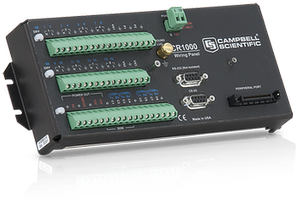
\includegraphics[width=100pt]{images/cr1000}
	\caption{Datalogger Campbell CR1000}
	\label{cr1000}
\end{figure}

Campbell Scientific es una compañía dedicada a la construcción y distribución de estos equipos. Junto con los equipos mantiene y provee un lenguaje de programación llamado CRBasic el cual está basado en \gloss{Basic}, mediante este lenguaje es posible crea diferentes scripts de control que permiten manejar el comportamiento del "datalogger", como es por ejemplo los datos provenientes de los diferentes sensores y el envío de datos a través de un módem celular o interfaz Ethernet. Las características principales de este "datalogger" son:

\begin{itemize}
\item Ideal para aplicaciones de medición solar, vientos, estaciones meteorológicas, calidad del aire, humedad del suelo, nivel de agua, prevenciones de avalanchas y otros.
\item Comunicación serial, dispone de entradas para dispositivos E/S.
\item Recolecta y almacena datos además puede controlar periféricos y actuar como sistema central.
\item Flexibilidad de alimentación energética y sistemas de comunicación, lo que lo hace ideal para instalaciones remotas.
\item 4 MB de memoria interna y puede ser expandido con módulos adicionales.
\item Soporta protocolos PakBus, Modbus, SDI-12, y DNP3.
\item Dispone de canales de expansión para periféricos lo que hace posible agregar funcionalidades al sistema.
\item Compatible con software LoggerNet, PC400, o ShortCut.
\item Protocolos de comunicación: TCP/IP, email, FTP, servidor web.
\item Entradas protegidas mediante tubos de descarga de gas(Gas Discharge Tube (GDT)).
\end{itemize}

\paragraph{Interfaz Ethernet NL200 Campbell}
Esta interfaz es un periférico distribuido por Campbell Scientific al igual que el "datalogger" mencionado anteriormente, que permite anexar una interfaz Ethernet directamente al "datalogger" de manera de lograr una conexión a la red Ethernet de manera directa(Fig:\ref{nl200}). Es mediante este aparato que la información recopilada de la Estación de monitoreo Fundaci'on Chile Vitacura envía los datos al servidor donde se alojan las aplicaciones desarrolladas y la base de datos.\\

\begin{figure}[h!]
        \centering
        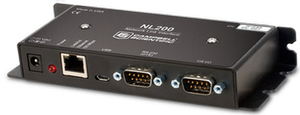
\includegraphics[width=100pt]{images/nl200}
        \caption{Periférico Campbell NL200}
	\label{nl200} 
\end{figure}

Como característica adicional hay que mencionar que es un periférico diseñado especialmente para funcionar con el Datalogger antes mencionado y además es un periférico pensado para un consumo de energía muy bajo, lo que lo hace ideal para estar conectado a la batería de la estación. Sus características principales son:

\begin{itemize}
\item Conector de corriente: DC Barrel.
\item Requerimientos de corriente: 7 to 20 Vdc. 
\item Consumo de corriente: 50 mA active @ 13 Vdc.
\item Standby forzado al tener 2 mA de corriente cuando esta conectado al puerto CS I/O en modo Bridge.
\item Rango de temperatura en operación : ${-25}^{\circ}$ to ${+50}^{\circ}C$.
\item Puede ser configurado a través de USB o Ethernet, mediante Telnet.
\item Puerto CS I/O: SDC 7, 8, 10, or 11.
\item Puerto RS-232: DTE.
\item Puerto USB: Micro-B.
\item Puerto Ethernet: IEEE 802.3, Auto-MDIX, IPv4, TCP, DHCP, Ping, Telnet, TLS, PakBus.
\item Dimensiones: 16 x 6.73 x 2.54 cm.
\item Peso: 177 g.
\item Puerto RS-232 DTE: 1200 hasta 115.2k bps.
\item Puerto CS I/O: 9600 hasta 460.8k bps.
\item Ethernet: 10/100 Mbps.
\end{itemize}

\paragraph{MultiModem Multitech modelo MTCBA-G-F4}
Este periférico construido y distribuido por Multitech es un módem que permite conectarse a una red GSM y/o GPRS. Este módem funciona en conjunto con el "datalogger" Campbell de la misma forma que lo hace el periférico NL200 salvo que este aparato provee al "datalogger" de una conexión a la Red de manera inalámbrica permitiendo conectar estaciones de monitores en lugares remotos del país(Fig:\ref{modem}).\\

\begin{figure}[h!]
        \centering
        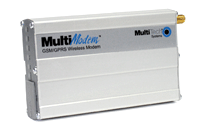
\includegraphics[width=100pt]{images/MultiModemGPRS}
        \caption{MultiModem Multitech MTCBA-G-F4}
	\label{modem} 
\end{figure}

Para poder operar con este módem es necesario tener contratado un plan de datos de telefonía móvil con alguna de las compañías que operan en el sector donde se instalan las estaciones de monitoreo. Sus características principales son:\\

\begin{itemize}
\item GPRS Clase 10.
\item Banda cuádruple GSM 850/900/1800/1900 MHz.
\item Corrección de errores MNP 2, Compresión V.42-bis.
\item Packet data up to 85.6K bps.
\item Pila TCP/IP embedida.
\item Conector de antena SMA.
\item 2 años de garantía.
\end{itemize}

\paragraph{Piranómetro PSP-Eppley}
El Piranómetro de Precisión Espectral es un instrumento de medición de clase mundial designado para medir la radiación entregada por el sol y la atmósfera, para todo el espectro eléctrico o bien puede configurarse para un segmento específico.\\
Se compone de una multi unión circular de hilo bobinado junto a una termopila Eppley que tiene la capacidad de soportar fuertes vibraciones y choques mecánicos(Fig:\ref{piranometro}).

\begin{figure}[h!]
        \centering
        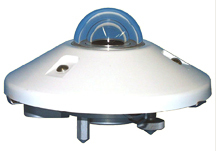
\includegraphics[width=100pt]{images/piranometro}
        \caption{Piranómetro psp-eplay}
	\label{piranometro}
\end{figure}

\paragraph{Sensor de temperatura y humedad HMP60}
Es una sonda de humedad sencilla, económica y duradera. Es adecuada para aplicaciones de volumen, integración en equipos de otros fabricantes, incubadoras, cajas de manipulación con guantes, invernaderos, cámaras de fermentación y registradoras de datos(Fig:\ref{hr}).

\begin{figure}[h!]
        \centering
        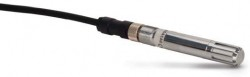
\includegraphics[width=100pt]{images/SensorThmp60}
        \caption{Sensor HMP60}
	\label{hr}
\end{figure}

\paragraph{Batería PS100}
Baterías de plomo-ácido, la fuente de alimentación cuenta con un regulador de carga, puertos libres con salidas DC 12V, además de un conector para el módulo fotovoltaico.

\begin{figure}[h!]
        \centering
        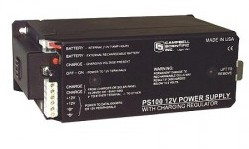
\includegraphics[width=100pt]{images/bateria}
        \caption{Batería PS100} 
\end{figure}

\paragraph{Panel fotovoltaico SX310M}
Modulo fotovoltaico de alta eficiencia, compuesto por celdas de nitrito de silicio multicristalinas.

\begin{figure}[h!]
        \centering
        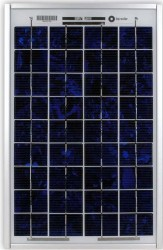
\includegraphics[width=100pt]{images/panelSolar}
        \caption{Panel Solar SX310M} 
\end{figure}

Sus características principales son:\\

\begin{itemize}
\item Tensión: 12.00 V.
\item Potencia: 10 W.
\item Corriente de salida: 0.59 mA.
\item Largo: 26.9 cm.
\item Alto: 42.1 cm.
\item Grosor: 2.3 cm.
\item Peso: 1.49 Kg.
\end{itemize}

\section{Diseño de la solución}
Basándonos en el análisis de la sección \ref{arquitectura} se diseño una solución de 3 componentes, las cuales podemos apreciar de manera mas clara en el Diagrama de Despliegue(Fig:\ref{despliegue}). Este diagrama detalla de manera precisa la implementación que tiene cada uno de los componentes.\\

\begin{figure}[h!]
        \centering
        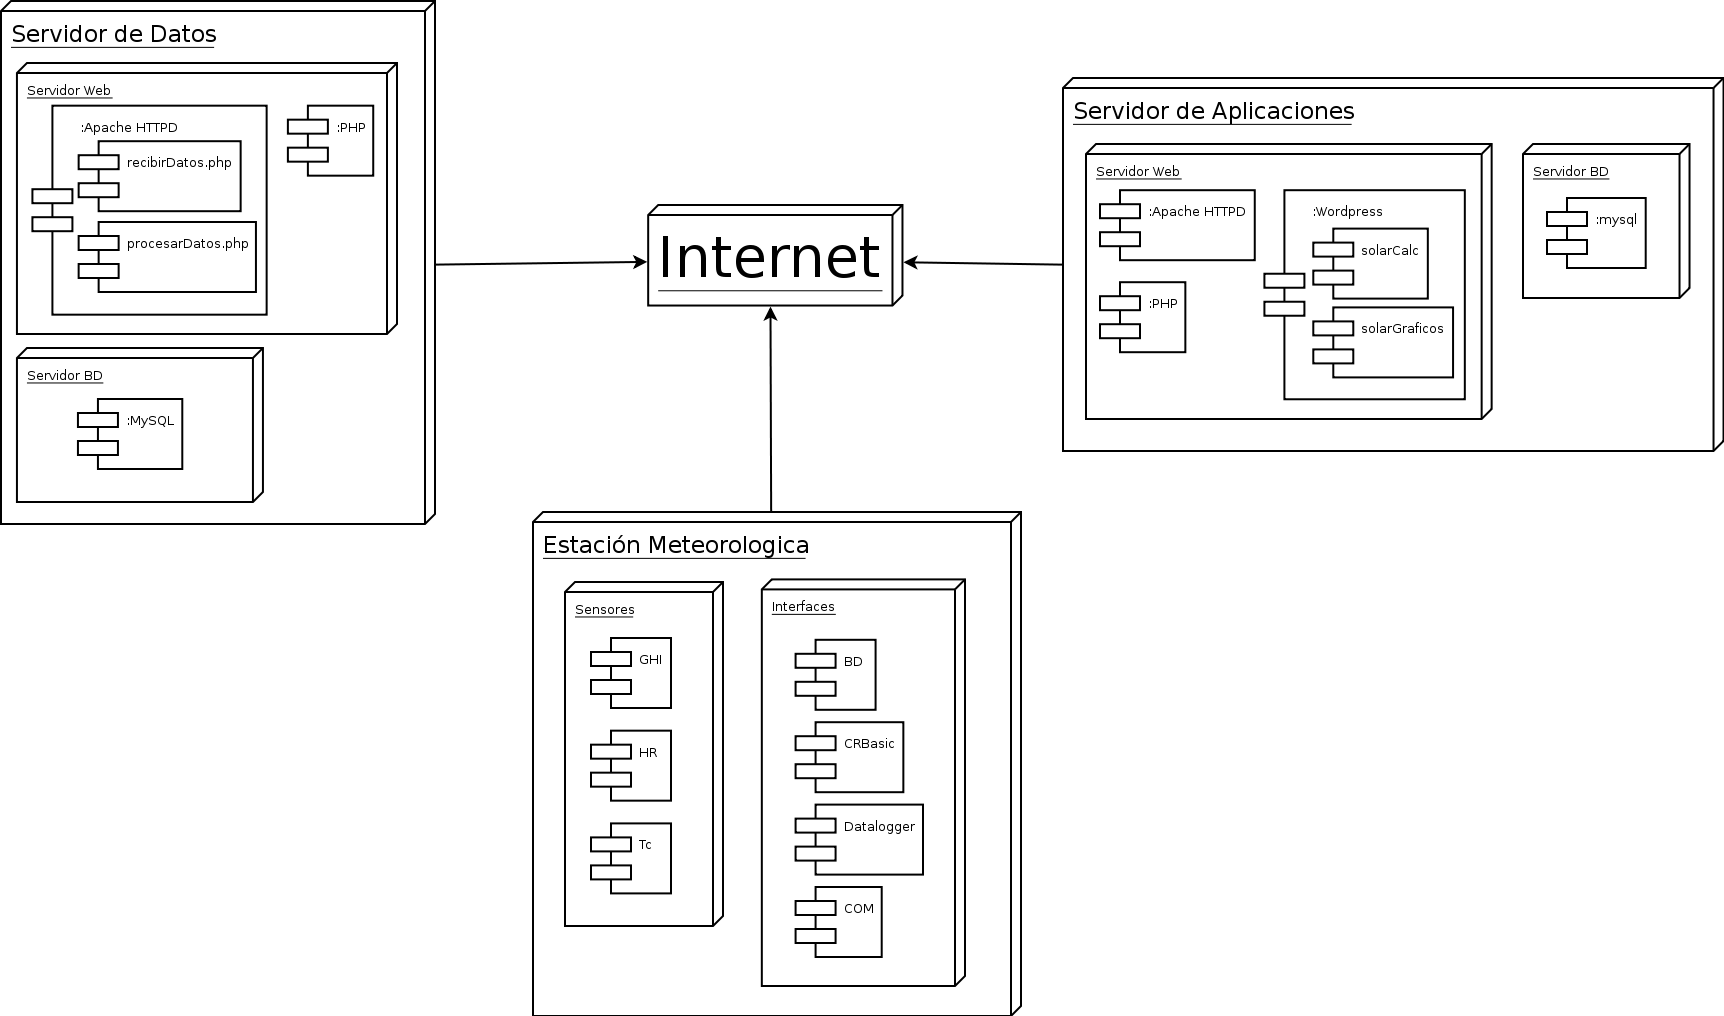
\includegraphics[scale=0.25]{images/despliegue}
        \caption{Diagrama de Despliegue}
	\label{despliegue} 
\end{figure}

\subsection{Aplicaciones}
En la componente de aplicaciones se distinguen 3 partes: Sitio Web de la RedSolLAC el cual fue desarrollado con anterioridad al inicio de esta memoria, la segunda parte es el modulo solarGraficos que permite visualizar los datos originados por las estaciones meteorológicas y la tercera parte el modulo solarCalc, el cual consiste en una calculadora para dimensionar sistemas fotovoltaicos, el cual utilizando el modulo de datos y los parámetros ingresados por el usuario entrega un informe de producción de energía.

\subsubsection{Sitio web RedSolLAC}
Inicialmente, antes de desarrollar esta memoria, RedSolLAC en su conformación desarrollo un sitio web el cual le proporciono una valiosa herramienta de difusión. RedSolLAC en un principio no requería de un sistema de publicación Web complejo, necesitaba un sistema que le permitiese de manera sencilla agregar nuevas publicaciones e información, así como de administrar la parte visual, estos requerimientos generaron la implementación del CMS Wordpress.\\
Posteriormente RedSolLAC se vio en la necesidad de implementar nuevas herramientas innovadoras que pudiesen generar curiosead en sus usuarios antiguos así como en los futuros usuarios que tendría el sitio.\\

Las características del sitio sobre el cual de implementan las mejoras planteadas en esta solución son:
\begin{table}[h!]
\caption{Características sitio Web RedSolLAC}
\begin{tabular}{| c | p{11cm} |}
        \hline
        \textbf{}  &       \textbf{}        \\
        \hline
	Wordpress&Versión 3.4.1\\
	\hline
	Theme(Perfil)&Revelation V1.0\\
	\hline
	Plugins&Contact(v0.7.1), Custom sidebars(v1.1), Google Analytics(v1.0.2), Maintenance Mode(v5.4), WordPress Google Form(v0.3), WordPress Importer(v0.6)\\
	\hline
	Hosting&Godaddy.com, Deluxe Linux, 150Mb, 500 Email, Ancho de banda ilimitado, 25 BD Mysql, DNS, 50 cuentas FTP\\
	\hline
	Base de datos&versión 5.0\\
	\hline
	PHP&Versión 5.2\\
	\hline
	Dominio&RedSolLAC.org\\
	\hline
\end{tabular}
\end{table}

\begin{figure}[h!]
        \centering
        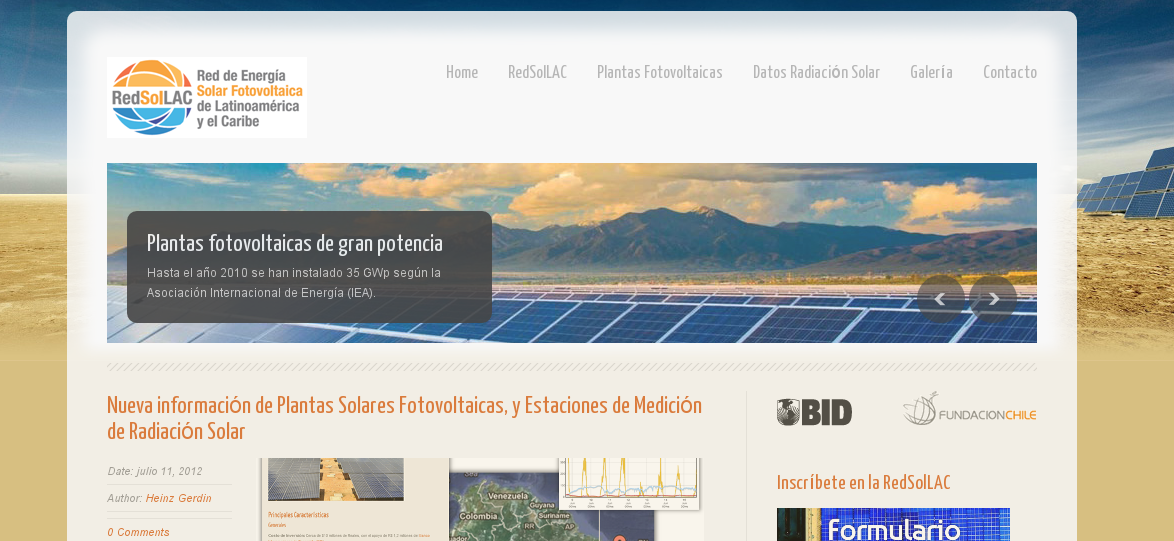
\includegraphics[scale=0.4]{images/webRedSolLAC}i
        \caption{Diagrama de Despliegue}
        \label{webRed}
\end{figure}

\subsubsection{SolarGraficos}
SolarGraficos es el nombre de la primera aplicación desarrollada en esta memoria y que cumple con los requerimientos de exponer los datos de manera sencilla e intuitiva los datos capturados por las estaciones meteorológicas en el sitio web de RedSolLAC. Esta aplicación fue desarrollada en PHP 5 y complementada con Javascript y jQuery, adicionalmente utiliza la librería Flot para crear un gráfico que incluye las mediciones individuales de los siguientes parámetros: la Redición Global Horizontal(GHI), la temperatura Ambiente(Tc) y la Humedad relativa del aire(HR).\\

La aplicación fue desarrollada siguiendo la estructura de programación de plugins de Wordpress\cite{aplicaciones:wplugins}, usando las funciones de la API que registran y eliminan gatilladores en tiempo de ejecución. El plugin creado registra una nueva pagina de Wordpress la cual utilizando una llamada ajax de la implementación de jquery solicita la ejecución del fichero php solarGrafico.php, este fichero contiene el código esencial que conforma la aplicación gráfica.

En primera instancia solarGrafico.php crea la estructura estática de la aplicación(Ver Fig:\ref{solarGraficoFoto2}) y escribe cierto código javascript que permite luego en tiempo de ejecución del lado del cliente hacer las llamadas necesarias que muestran los datos solicitados(Ver Fig:\ref{solarGraficoS}). Una vez creada la estructura de la calculadora se solicita al Servidor de Almacenamiento de datos mediante una consulta ajax sincrónica por los datos del día, el cual es el periodo por defecto. {una vez estos datos están completamente cargados, la aplicación crea un gráfico por defecto que contienen las 3 curvas mencionadas con anterioridad(GHI, HR y Tc) en el periodo del día actual, luego de crear el gráfico se cargan las barras que muestran la ultima lectura de cada curva y el modulo de descarga de datos. Finalizada esta carga inicial el sistema ejecuta 3 llamadas ajax sincrónicas(Ver Fig:\ref{solarGraficoE}) al Servidor de Almacenamiento de Datos solicitando datos de los periodos correspondientes a una semana, un mes y un año tomando como referencia la fecha actual. a medida que los datos se cargan la opción de visualizar dicho periodo va estando disponible en la interfaz de usuario(Ver Fig:\ref{solarGraficoFoto1}) para que este pueda solicitar ser graficada. Debido a que las llamadas para cargar los datos de los periodos de tiempo mas extensos son llamadas asincronicas el navegador no se bloquea y el usuario puede seguir utilizando la aplicación mientras que estos datos están cargados.

\begin{figure}[h!]
        \centering
        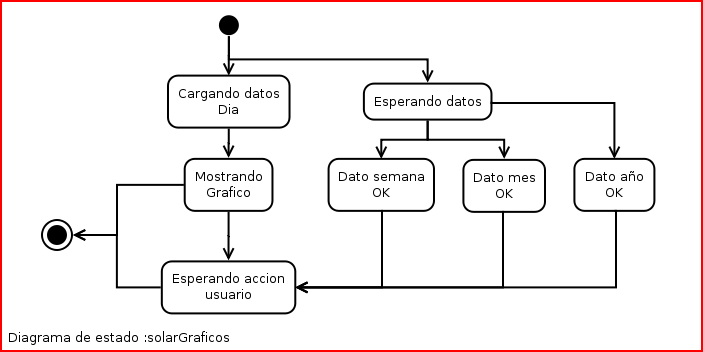
\includegraphics[scale=0.4]{images/graficosEstados}
        \caption{Diagrama de Estados solarGraficos}
        \label{solarGraficoE}
\end{figure}
\begin{figure}[h!]
        \centering
        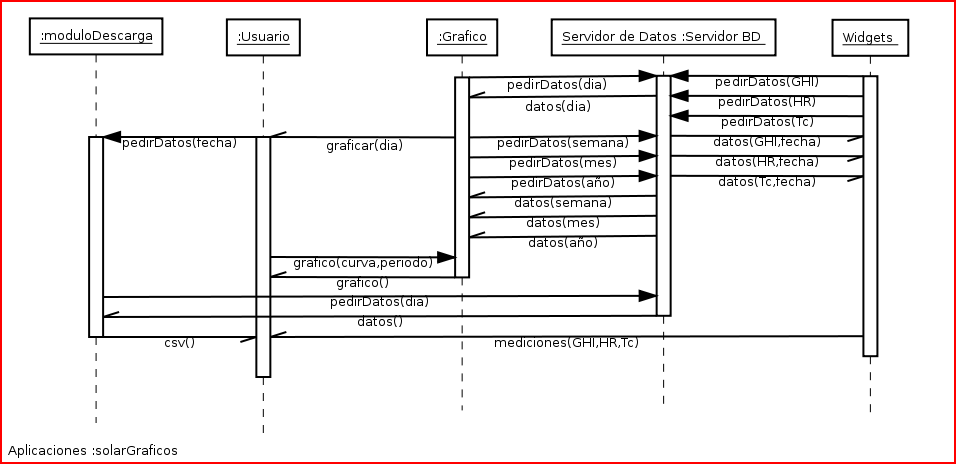
\includegraphics[scale=0.4]{images/graficosSecuencia}i
        \caption{Diagrama de Secuencia solarGraficos}
        \label{solarGraficoS}
\end{figure}

\begin{figure}[h!]
        \centering
        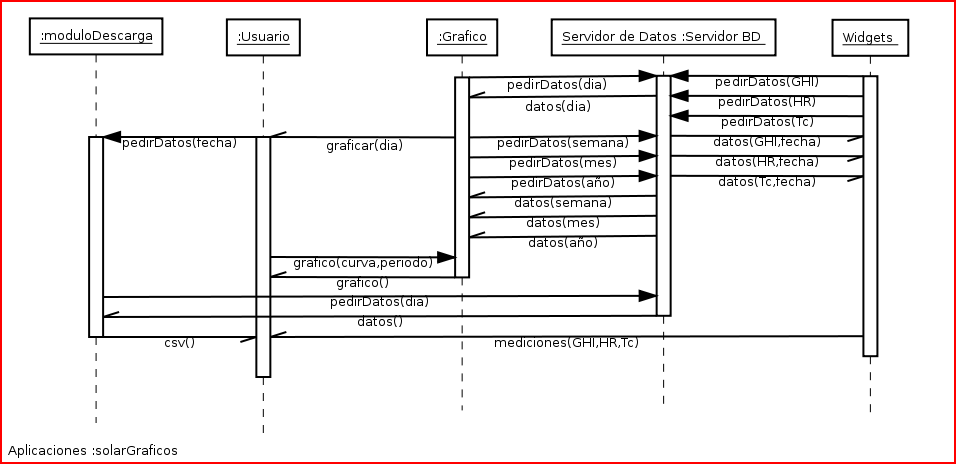
\includegraphics[scale=0.4]{images/graficosSecuencia}
        \caption{Imagen de la aplicacion SolarGraficos - Cargando datos}
        \label{solarGraficoFoto1}
\end{figure}
\begin{figure}[h!]
        \centering
        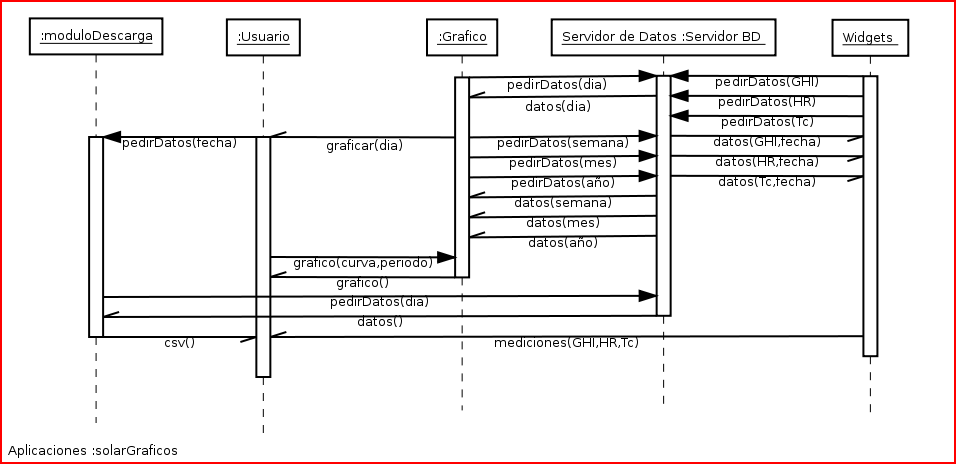
\includegraphics[scale=0.4]{images/graficosSecuencia}
        \caption{Imagen de la aplicación SolarGraficos - Estructura}
        \label{solarGraficoFoto2}
\end{figure}

\subsubsection{SolarCalc}

\subsection{Estaciones}
El componente Estaciones abarca todas las estaciones de medicion que están adaptadas para registrar datos en la componente de almacenamiento de datos, para ello fue necesario acondicionar cada estación y agregarles un modulo de comunicación, este modulo de comunicación depende del lugar geográfico donde se ubica la estación ya que esto determinara la tecnología que este modulo implementara, cualquiera sea la tecnología el sistema fue diseñado para que cada estación se conecte a internet y a través de esta red pueda libremente acceder al modulo de almacenamiento de datos. Adicionalmente y para dar cumplimiento a los requerimientos de seguridad y resguardo de datos ante posibles fallas fue necesario programar el modulo para que pudiese almacenar datos de manera local independiente del estado de la conexión, diseñando un protocolo manual de restauración de datos.

Principalmente Fundación Chile ofrece a sus clientes dos tipos de estaciones, Serie Dédalo y serie Icaro,cada una de ellas tienen componentes diferentes y fueron diseñadas para diferentes requerimientos de clientes, las especificaciones generales de cada una de las Series se encuentran en la sección de anexos, Dédalo(Ver:\ref{dedalo}) e Icaro(Ver:\ref{icaro}). Para realizar las pruebas del sistema se utilizo una estación Serie Dédalo, las características especificas de esta estación se presentan en el cuadro siguiente(Ver:\ref{estacionPrueba}):

\begin{table}[h!]
\label{estacionPrueba}
\caption{Tabla de requerimientos funcionales}
\begin{tabular}{| c | p{11cm} |}
        \hline
        \textbf{Requerimiento}  &       \textbf{Detalle}        \\
        \hline
\end{tabular}
\end{table}

Para que dicha estación opere de manera correcta es necesario programar su Datalogger con el siguiente script:

(explicaion del script)

Para graficar de mejor manera cual es el comportamiento de la estación dentro de este componente del sistema se presenta un diagrama de estados y un diagrama de secuencia del comportamiento que tienen cada una de las estaciones.

\begin{figure}[h!]
        \centering
        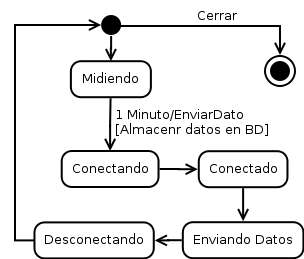
\includegraphics[scale=0.25]{images/estacionEstados}
        \caption{Diagrama de Estado estación meteorológica}
        \label{despliegue}
\end{figure}

(explicación diagrama)

\begin{figure}[h!]
        \centering
        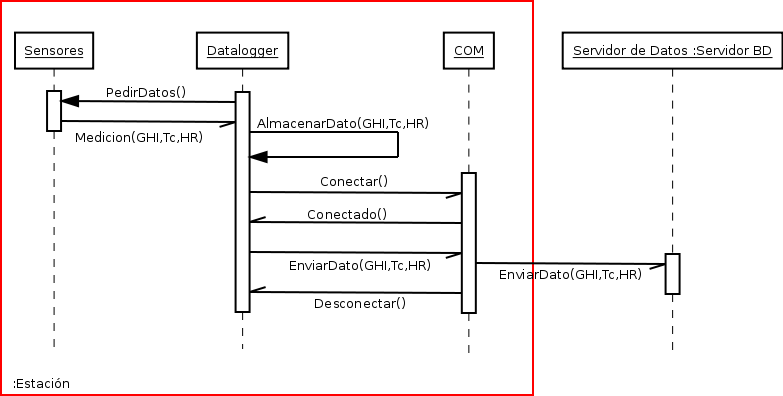
\includegraphics[scale=0.25]{images/estacionSecuencia}
        \caption{Diagrama de Secuencia estación meteorológica}
        \label{despliegue}
\end{figure}

(explicación diagrama)

\subsection{Almacenamiento de datos}
El componente de almacenamiento de datos era inexistente, anterior al desarrollo de este sistema cada estación almacenaba datos en su memoria interna y era necesario que una persona accediera físicamente a cada estación, ésta apoyado con un pc portatil se conectaba a las estaciones y descargaba los datos. Este proceso resultaba bastante complejo y en varias ocasiones se perdían datos. Este módulo se compone de un servidor de bases de datos y un servidor Web el cual contiene scripts necesarios para el manejo y mantención de la base de datos, así como proporcionar un acceso seguro para que las estaciones registren sus datos.\\

El sistema de Almacenamiento de datos esta compuesto por un solo servidor el cual implementa el servidor Web Apache HTTPD y el servidor de bases de datos MySQL, el servicio MySQL se encarga directamente de almacenar los datos en bruto que llegan desde las estaciones y atender las solicitudes de datos del componente de aplicaciones mientras que el servicio Web implementa ciertas rutinas escritas en PHP que aportan al sistema de seguridad e integridad de los datos así como a la mantención de los datos, adicionalmente implementa rutinas que forman parte del sistema de respaldo manual que incorpora la componente para casos de perdida de conexión.\\ Uno de los requerimientos claves de este sistema es la robustas y la integridad de los datos, así como la confiabilidad de ellos. Este sistema tiene restringido el ingreso de datos solo al modulo de estaciones y en ocasiones especiales al sistema de mantenimiento manual, por lo que implementa rutinas en PHP a revés del servidor Web que impiden que cualquier actor diferente de una estación pueda registrar datos nuevos. Estas rutinas son ejecutadas directamente por las estaciones a trabes del datalogger haciendo llamadas GET con ciertas llaves de seguridad.\\
El sistema implementa una salida de datos libre, esto quiere decir que cualquiera que te posea acceso a la base de datos puede solicitar el envió de estos a sus aplicaciones sin la necesidad de llaves extras de seguridad. Para el caso especifico de este sistema son algunos elementos de la componente te aplicaciones quienes hacen estas solicitudes.\\

Cuándo una estación hace una llamada GET, el servidor Web mediante una rutina en PHP verifica las llaves de seguridad, verifica los datos que le son enviados de la estación y luego los envía a la base de datos, una vez que la petición GET es recibida esta devuelve a la estación un mensaje 200 si la llamada fue recibida o un mensaje 404 si la llamada no fue recibida. En cualquier caso para el datalogger es indiferente si la petición fue aceptada o no ya que el datalogger implementa su propia base de datos local a modo de respaldo. Una ves que la estación entrega los datos al sistema de almacenamiento esta tampoco tienen la posibilidad de verificar si estos fueron almacenados correctamente.

\begin{figure}[h!]
        \centering
        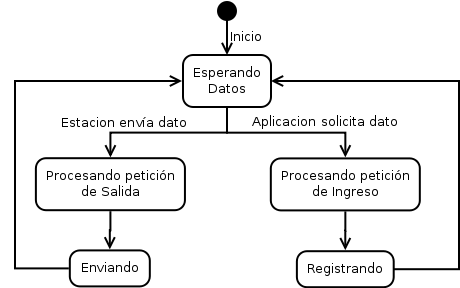
\includegraphics[scale=0.25]{images/datosEstados}
        \caption{Diagrama de Estados Sistema de Almacenamiento}
        \label{almacenamientoSecuencia}
\end{figure}

